\begin{figure}[!htbp]
\centering
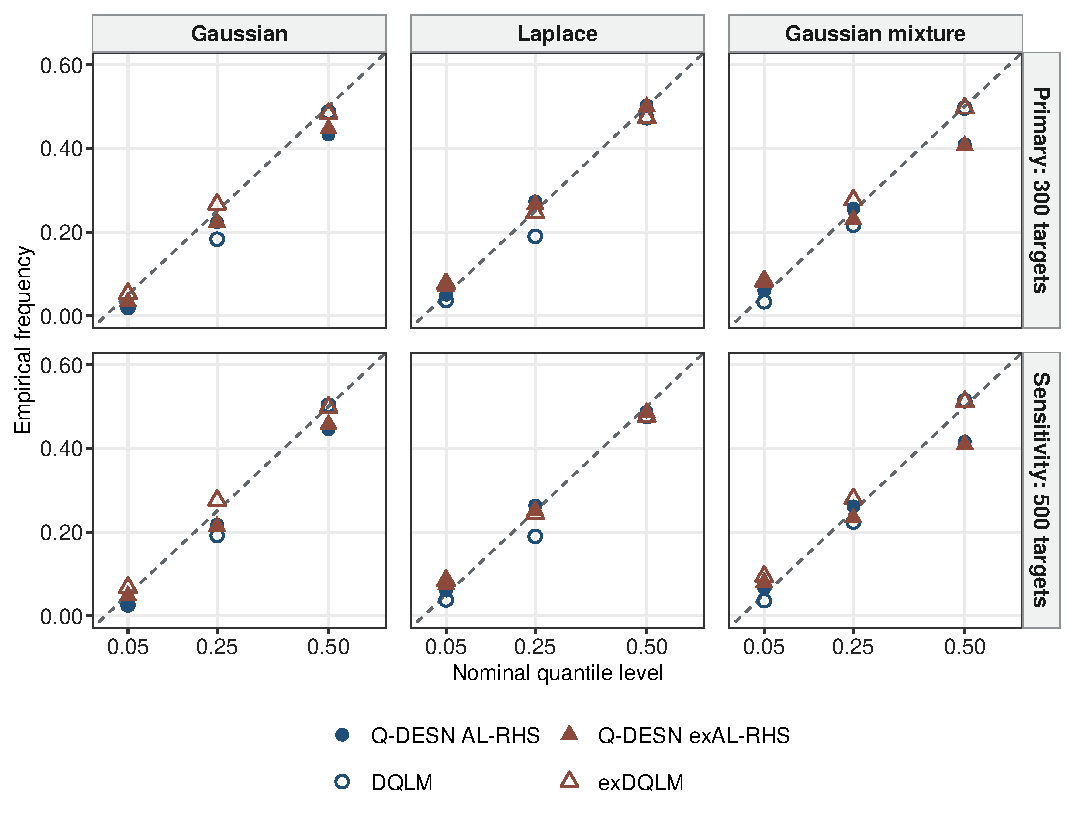
\includegraphics[width=0.98\textwidth]{figures/independent_simulation/independent_forecast_calibration_v1.pdf}
\caption{Empirical quantile frequencies for the check-loss-selected specifications over the 300-target primary period and its 500-target extension. At each target, the reported quantile is the median of the pooled posterior location draws. Each point gives the fraction of observed responses at or below that forecast; the dashed diagonal marks the nominal probability. Colours and symbols follow the forecast-score figures. Each probability level uses its corresponding quantile-centred response series. Frequencies summarize the fixed evaluation record; no sampling confidence bands are shown.}
\figalt{Six panels compare empirical response frequencies below posterior-median quantile forecasts with the nominal levels 0.05, 0.25 and 0.50, for four models, three error families and two evaluation periods.}
\label{fig:supp-independent-quantile-calibration}
\end{figure}
